\documentclass[11pt]{article}
\usepackage[margin=0.75in]{geometry}
\usepackage{amsmath}
\usepackage{enumitem}
\usepackage{tikz,soul}

\usepackage{multicol}

\newcommand{\ds}{\displaystyle}

\begin{document}
\newcounter{enumCount}
\pagestyle{empty}
\subsection*{Math 105 - Homework 5 \hfill Name: \underline{\hspace*{2in}}}


\noindent 
\textit{In each problem below, find an equation for the line that fits the description.}
\begin{multicols}{2}
\begin{enumerate}
\setcounter{enumi}{\theenumCount}
\item Passes through $(1,-2)$ and $(3,4)$.
\item Passes through $(-4,5)$ and $(8,2)$ 
\setcounter{enumCount}{\theenumi}
\end{enumerate}
\end{multicols}
\vfill




\begin{multicols}{2}
\begin{enumerate}
\setcounter{enumi}{\theenumCount}
\item Has a slope of 5 and crosses the $x$-axis at $x=3$.
\item Passes through $(3,4)$ with slope of $-6$.
\setcounter{enumCount}{\theenumi}
\end{enumerate}
\end{multicols}
\vfill


\begin{enumerate}
\setcounter{enumi}{\theenumCount}
\item Find the slope and $y$-intercept of the line $4x + 6y = 24$.
\vfill


\item Suppose that there are 4 inches of snow already on the ground when a new snow storm arrives.  During the storm, snow falls at a rate of 2/3 of an inch per hour.  
\begin{enumerate}
\item Find a formula for the depth of the snow on the ground ($y$) as a function of the number of hours ($x$) that have passed since the storm started. 
\vfill

\item At this rate, how long would it be until the snow is 1 foot (12 inches) deep?  
\vfill
\end{enumerate}

\item Suppose that $p(x) = x^2 - 8x + 12$. Find the roots of $p(x)$, then sketch a graph of $y = p(x)$.  Be sure to label the coordinates of the vertex and the points where the graph crosses the x and y-axes. 
\vfill

\item Find the $x$-values where the line $y = 2x + 5$ intersects the parabola $y^2 - 3$. 
\vfill


\newpage

\item Find the $x$-values where the parabolas $y = 2x^2 - 5x - 3$ and $y = -x^2 + 4x + 9$ cross. 
\vfill

\item Suppose that a ball thrown into the air follows a parabolic trajectory with its height above the ground (in meters) obeying the formula $h(x) = -0.1x^2 + 0.7x + 0.6$ where $x$ is the horizontal distance of the ball from the thrower.  Find the roots and the vertex of this parabola.  
\vfill


\setcounter{enumCount}{\theenumi}
\end{enumerate}

\noindent
\textit{Sketch graphs of the following equations.  Be sure to label points where the graphs cross the $x$ and $y$-axes.}

\begin{multicols}{2}
\begin{enumerate}
\setcounter{enumi}{\theenumCount}
\item $y = \tfrac{1}{2}x - 3$ \\
\begin{center}
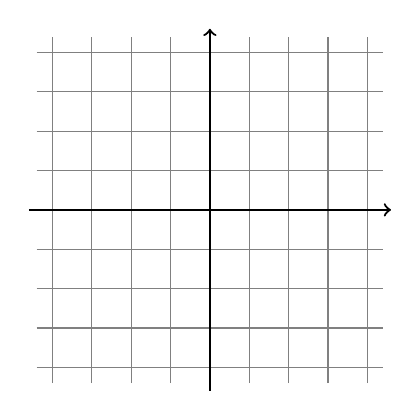
\begin{tikzpicture}
\draw[scale=0.5, thin, gray] (-4.4,-4.4) grid (4.4,4.4);
\draw[thick,->] (-2.3,0) -- (2.3,0);
\draw[thick,->] (0,-2.3) -- (0,2.3);
\end{tikzpicture}
\end{center}

\item $y = \dfrac{x^2 - 2x - 8}{4}$ \\
\begin{center}
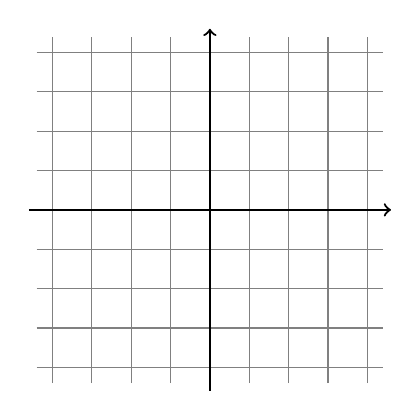
\begin{tikzpicture}
\draw[scale=0.5, thin, gray] (-4.4,-4.4) grid (4.4,4.4);
\draw[thick,->] (-2.3,0) -- (2.3,0);
\draw[thick,->] (0,-2.3) -- (0,2.3);
\end{tikzpicture}
\end{center}
\setcounter{enumCount}{\theenumi}
\end{enumerate}
\end{multicols}


\begin{multicols}{2}
\begin{enumerate}
\setcounter{enumi}{\theenumCount}
\item $3y - 2x = 6$ \\
\begin{center}
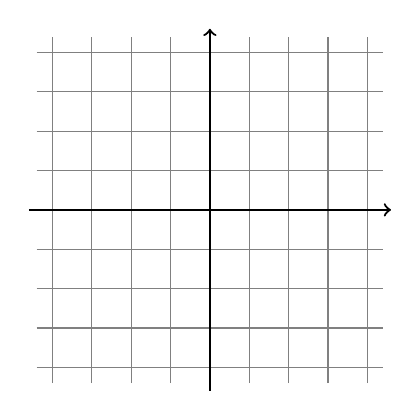
\begin{tikzpicture}
\draw[scale=0.5, thin, gray] (-4.4,-4.4) grid (4.4,4.4);
\draw[thick,->] (-2.3,0) -- (2.3,0);
\draw[thick,->] (0,-2.3) -- (0,2.3);
\end{tikzpicture}
\end{center}

\item $y = -(x+1)^2$ \\
\begin{center}
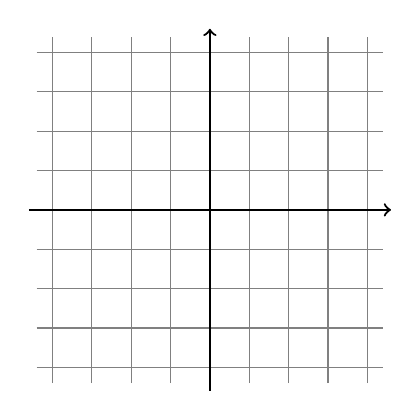
\begin{tikzpicture}
\draw[scale=0.5, thin, gray] (-4.4,-4.4) grid (4.4,4.4);
\draw[thick,->] (-2.3,0) -- (2.3,0);
\draw[thick,->] (0,-2.3) -- (0,2.3);
\end{tikzpicture}
\end{center}
\setcounter{enumCount}{\theenumi}
\end{enumerate}
\end{multicols}

\end{document}
